
%(BEGIN_QUESTION)
% Copyright 2006, Tony R. Kuphaldt, released under the Creative Commons Attribution License (v 1.0)
% This means you may do almost anything with this work of mine, so long as you give me proper credit

A {\it microcontroller} is a single-chip digital computer with onboard I/O capable of receiving and transmitting different types of electrical signals, and a processor capable of executing a series of written instructions.  This one is being used to control an air compressor:

$$\includegraphics[width=15.5cm]{i01454x01.eps}$$

Examine the following program (written in an informal programming language called ``pseudocode'') and explain how the microcontroller decides when to turn the motor on and off.  Also determine the pressures at which the microcontroller turns on and shuts off the compressor:

\vskip 10pt

\hbox{ \vrule
\vbox{ \hrule \vskip 3pt
\hbox{ \hskip 3pt
\vbox{ \hsize=5in \raggedright

\noindent
\underbar{\bf Pseudocode listing}

\vskip 10pt

{\tt Declare Pin0 as an analog input (scale 0 to 5 volts = 0 to 1023)}

{\tt Declare Pin1 as a discrete output}

{\tt Declare Pin2 as a discrete output}

{\tt Declare A as a constant = 805}

{\tt Declare B as a constant = 750}

{\tt Declare C as a constant = 700}

\vskip 10pt

{\tt LOOP}

\hskip 10pt {\it // (Comment: Motor control points)}

\hskip 10pt {\tt IF Pin0 > A, SET Pin1 LOW}

\hskip 10pt {\tt ELSEIF Pin0 < B, SET Pin1 HIGH}

\hskip 10pt {\tt ENDIF}

\vskip 10pt

\hskip 10pt {\it // (Comment: Alarm LED control points)}

\hskip 10pt {\tt IF Pin0 < C, SET Pin2 HIGH}

\hskip 10pt {\tt ELSE SET Pin2 LOW}

\hskip 10pt {\tt ENDIF}

{\tt ENDLOOP}
}
\hskip 3pt}%
\vskip 5pt \hrule}%
\vrule}

\vskip 20pt \vbox{\hrule \hbox{\strut \vrule{} {\bf Suggestions for Socratic discussion} \vrule} \hrule}

\begin{itemize}
\item{} Which sections of the pseudocode program listing are executed repeatedly, and which sections are executed only once?
\item{} How many bits of resolution does this microcontroller have for the analog input on pin \#0, assuming that 0 to 1023 is the full range of the converter?
\item{} Explain how the {\it solid state relay} device works to help control the compressor motor.
\item{} Explain what would happen if you deleted the {\tt LOOP} and {\tt ENDLOOP} statements in the microcontroller program.
\item{} Modify the pseudocode so that the alarm LED comes on if the pressure gets too high.
\item{} Modify the pseudocode so that the alarm LED comes on if the pressure gets too high {\it or} too low.
\end{itemize}

\underbar{file i01454}
%(END_QUESTION)





%(BEGIN_ANSWER)

{\tt A} = {\tt 805} = 110 PSI (motor stop point)

{\tt B} = {\tt 750} = 100 PSI (motor start point)

{\tt C} = {\tt 700} = 90.8 PSI (low air pressure alarm point)

%(END_ANSWER)





%(BEGIN_NOTES)

The pressure transmitter measures 0 to 150 PSI and outputs 4 to 20 mA.  That current, passing through a 250 ohm resistor, creates a 1 to 5 volt signal for the microcontroller's ADC to read (as a numerical count value ranging as high as 1023 counts).

\vskip 10pt

The LRV (1 volt) generates a count value of 205 counts ($1 \over 5$ of 1023).  Therefore, 205 to 1023 represents 0 to 150 PSI.  The count values specified in the program correspond to the following pressures:

\begin{itemize}
\item{} $A$ = 805 counts = ${805 \over 1023} \times 5$ = 3.9345 volts = 110.04 PSI
\vskip 5pt
\item{} $B$ = 750 counts = ${750 \over 1023} \times 5$ = 3.6657 volts = 99.96 PSI
\vskip 5pt
\item{} $C$ = 700 counts = ${700 \over 1023} \times 5$ = 3.4213 volts = 90.80 PSI
\end{itemize}

The compressor motor stops when the pressure exceeds $A$ (110.04 PSI), and re-starts when it falls below $B$ (99.96 PSI).  An alarm bit is set if the pressure is less than $C$ (90.80 PSI).

\vskip 10pt

$2^{10} = 1024$, so this must be a 10-bit ADC.









\vskip 20pt \vbox{\hrule \hbox{\strut \vrule{} {\bf Virtual Troubleshooting} \vrule} \hrule}

This question is a good candidate for a ``Virtual Troubleshooting'' exercise.  Presenting the diagram to students, you first imagine in your own mind a particular fault in the system.  Then, you present one or more symptoms of that fault (something noticeable by an operator or other user of the system).  Students then propose various diagnostic tests to perform on this system to identify the nature and location of the fault, as though they were technicians trying to troubleshoot the problem.  Your job is to tell them what the result(s) would be for each of the proposed diagnostic tests, documenting those results where all the students can see.

During and after the exercise, it is good to ask students follow-up questions such as:

\begin{itemize}
\item{} What does the result of the last diagnostic test tell you about the fault?
\item{} Suppose the results of the last diagnostic test were different.  What then would that result tell you about the fault?
\item{} Is the last diagnostic test the best one we could do?
\item{} What would be the ideal order of tests, to diagnose the problem in as few steps as possible?
\end{itemize}

%INDEX% Control, basics: on/off control (implemented in a microcontroller)

%(END_NOTES)


